\documentclass[12pt, titlepage]{article}

\usepackage{fullpage}
\usepackage[round]{natbib}
\usepackage{multirow}
\usepackage{booktabs}
\usepackage{tabularx}
\usepackage{graphicx}
\usepackage{float}
\usepackage{hyperref}
\hypersetup{
    colorlinks,
    citecolor=blue,
    filecolor=black,
    linkcolor=red,
    urlcolor=blue
}

%% Comments

\usepackage{color}

\newif\ifcomments\commentstrue %displays comments
%\newif\ifcomments\commentsfalse %so that comments do not display

\ifcomments
\newcommand{\authornote}[3]{\textcolor{#1}{[#3 ---#2]}}
\newcommand{\todo}[1]{\textcolor{red}{[TODO: #1]}}
\else
\newcommand{\authornote}[3]{}
\newcommand{\todo}[1]{}
\fi

\newcommand{\wss}[1]{\authornote{blue}{SS}{#1}} 
\newcommand{\plt}[1]{\authornote{magenta}{TPLT}{#1}} %For explanation of the template
\newcommand{\an}[1]{\authornote{cyan}{Author}{#1}}

%% Common Parts

\newcommand{\progname}{MTOBridge} % PUT YOUR PROGRAM NAME HERE
\newcommand{\authname}{Team 15, Alpha Software Solutions
\\ Badawy, Adham
\\ Yazdinia, Pedram
\\ Jandric, David
\\ Vakili, Farzad
\\ Vezina, Victor
\\ Chiu, Darren} % AUTHOR NAMES                  

\usepackage{hyperref}
    \hypersetup{colorlinks=true, linkcolor=blue, citecolor=blue, filecolor=blue,
                urlcolor=blue, unicode=false}
    \urlstyle{same}


\newcounter{acnum}
\newcommand{\actheacnum}{AC\theacnum}
\newcommand{\acref}[1]{AC\ref{#1}}

\newcounter{ucnum}
\newcommand{\uctheucnum}{UC\theucnum}
\newcommand{\uref}[1]{UC\ref{#1}}

\newcounter{mnum}
\newcommand{\mthemnum}{M\themnum}
\newcommand{\mref}[1]{M\ref{#1}}

\begin{document}

\title{Module Guide for \progname{}} 
\author{\authname}
\date{\today}

\maketitle

\pagenumbering{roman}

\section{Revision History}

\begin{tabularx}{\textwidth}{p{3cm}p{4cm}X}
\toprule {\bf Date} & {\bf Developer(s)} & {\bf Notes}\\
\midrule
2023-01-17& Adham & Added Sections 4,5,7, and 8\\
2023-01-17& Farzad & Added Introduction\\
2023-01-17& Victor & Added Use Hierarchy\\
2023-04-4& Pedram & Rev1 Changes\\
\bottomrule
\end{tabularx}

\newpage

\section{Reference Material}

This section records information for easy reference.

\subsection{Abbreviations and Acronyms}

\renewcommand{\arraystretch}{1.2}
\begin{tabular}{l l} 
  \toprule		
  \textbf{symbol} & \textbf{description}\\
  \midrule 
  AC & Anticipated Change\\
  CHBDC & Canadian Highway Bridge Design Code\\
  DAG & Directed Acyclic Graph \\
  M & Module \\
  MG & Module Guide \\
\progname & A portable Software program capable of helping bridge engineers\\
  OS & Operating System \\
  R & Requirement\\
  SC & Scientific Computing \\
  SRS & Software Requirements Specification\\
  UC & Unlikely Change \\
  \bottomrule
\end{tabular}\\

\newpage

\tableofcontents

\listoftables

\listoffigures

\newpage

\pagenumbering{arabic}

\section{Introduction}

Decomposing a system into modules is a commonly accepted approach to developing
software.  A module is a work assignment for a programmer or programming
team~\citep{ParnasEtAl1984}.  We advocate a decomposition
based on the principle of information hiding~\citep{Parnas1972a}.  This
principle supports design for change because the ``secrets'' that each module
hides represent likely future changes.  Design for change is valuable in SC,
where modifications are frequent, especially during initial development as the
solution space is explored.  

Our design follows the rules laid out by \citet{ParnasEtAl1984}, as follows:
\begin{itemize}
\item System details that are likely to change independently should be the
  secrets of separate modules.
\item Each data structure is implemented in only one module.
\item Any other program that requires information stored in a module's data
  structures must obtain it by calling access programs belonging to that module.
\end{itemize}

After completing the first stage of the design, the Software Requirements
Specification (SRS), the Module Guide (MG) is developed~\citep{ParnasEtAl1984}. The MG
specifies the modular structure of the system and is intended to allow both
designers and maintainers to easily identify the parts of the software.  The
potential readers of this document are as follows:

\begin{itemize}
\item New project members: This document can be a guide for a new project member
  to easily understand the overall structure and quickly find the
  relevant modules they are searching for.
\item Maintainers: The hierarchical structure of the module guide improves the
  maintainers' understanding when they need to make changes to the system. It is
  important for a maintainer to update the relevant sections of the document
  after changes have been made.
\item Designers: Once the module guide has been written, it can be used to
  check for consistency, feasibility, and flexibility. Designers can verify the
  system in various ways, such as consistency among modules, the feasibility of the
  decomposition, and flexibility of the design.
\end{itemize}

\subsection{System Purpose}
This project aims to develop an application MTOBridge that leverages novel bridge analysis methods and better visualizes their outputs while enhancing the user experience.
This enables the refined methods of analysis to become routine for bridge design and evaluation. Moreover, A unique feature of MTOBridge which is otherwise unavailable in other
bridge design/evaluation software, is that a direct comparison can be obtained between the results obtained from the CHBDC approximate/simplified approach and those from the
refined analysis. This endeavor will facilitate confidence in using refined analysis for bridge evaluation and design.

\subsection{Document Purpose}
The Purpose of this document is to demonstrate how the system is decomposed into modules and communicate the overall design of the system which satisfies the requirements
 mentioned in the SRS. As a result helping future project members, maintainers, and designers to easily identify the parts of the software.

\subsection{System Scope}
The system is meant for use in offices (including home offices) by civil engineers designing or retrofitting bridges.

\subsection{Document Scope}
The scope of this document includes modules created by the development team and not components provided by the stakeholder (such as the MATLAB engines) 
or third-party libraries.

The rest of the document is organized as follows. Section
\ref{SecChange} lists the anticipated and unlikely changes of the software
requirements. Section \ref{SecMH} summarizes the module decomposition that
was constructed according to the likely changes. Section \ref{SecConnection}
specifies the connections between the software requirements and the
modules. Section \ref{SecMD} gives a detailed description of the
modules. Section \ref{SecTM} includes two traceability matrices. One checks
the completeness of the design against the requirements provided in the SRS. The
other shows the relation between anticipated changes and the modules. Section
\ref{SecUse} describes the use relation between modules.

\section{Anticipated and Unlikely Changes} \label{SecChange}

This section lists possible changes to the system. According to the likeliness
of the change, the possible changes are classified into two
categories. Anticipated changes are listed in Section \ref{SecAchange}, and
unlikely changes are listed in Section \ref{SecUchange}.

\subsection{Anticipated Changes} \label{SecAchange}

Anticipated changes are the source of the information that is to be hidden
inside the modules. Ideally, changing one of the anticipated changes will only
require changing the one module that hides the associated decision. The approach
adapted here is called design for
change.

\begin{enumerate}
    \item How the set of backend MATLAB functions will be called
    \item How the calculation call will be visualized
    \item The format of the truck platoon input data
    \item How the truck platoon input data is stored
    \item The method of visualizing the truck platoon configuration
    \item The method of visualizing the truck platoon data saving
    \item The method of visualizing the truck platoon data loading
    \item The format of the bridge input data
    \item How the bridge input data is stored
    \item The method of visualizing the bridge configuration
    \item The method of visualizing the bridge data saving
    \item The method of visualizing the bridge data loading
    \item How the solver configuration data is stored
    \item The method of visualizing the solver configuration
    \item The format of the solver configuration data
    \item How the concerned section specification data is stored
    \item How the critical section specification data is stored
    \item The method of visualizing the solver configuration data saving
    \item The method of visualizing the solver configuration data loading
    \item How data is saved to the file system 
    \item How data is loaded from the file system 
    \item The format of the output report created by the program
    \item The method by which the Output Report is visualized for the user
    \item How the output report data is stored
    \item The method of visualizing the output report saving
    \item The set of backend MATLAB calculations called by the program
\end{enumerate}    

\subsection{Unlikely Changes} \label{SecUchange}

The module design should be as general as possible. However, a general system is
more complex. Sometimes this complexity is not necessary. Fixing some design
decisions at the system architecture stage can simplify the software design. If
this decision should later need to be changed, then many parts of the design
will potentially need to be modified. Hence, it is not intended that these
decisions will be changed.

\begin{itemize}
    \item The language the backend calculations are written in
    \item The operating system the program will run on
    \item The input/output devices available to the user
    \item The baseline level of technical knowledge of the users of the software
    \item The primary functions of the software (i.e, visually and textually representing the results of forces imparted on some bridge by some truck platoon)
    \item The publicity of the software (expected to be a private in-house software used only by the MTO)
    \item The number of solvers available to choose between
\end{itemize}

\section{Module Hierarchy} \label{SecMH}

This section provides an overview of the module design. Modules are summarized
in a hierarchy decomposed by secrets. The modules listed
below, which are leaves in the hierarchy tree, are the modules that will
actually be implemented. For clarity, The three top level categories as well and all leaf nodes are bolded.

\begin{enumerate}
    \item[|] \textbf{Hardware Hiding}
    \begin{enumerate}
        \item[|] Data Storage Hiding
        \begin{enumerate}
            \item[|] Input Data Storage Hiding
            \begin{enumerate}
                \item[|] \textbf{Truck Platoon Configuration Data Storage Hiding}
                \item[|] \textbf{Bridge Configuration Data Storage Hiding}
            \end{enumerate}
            \item[|] Calculation Data Storage Hiding
            \begin{enumerate}
                \item[|] Calculation Variable Data Storage Hiding
                \begin{itemize}
                    \item[|] \textbf{Solver Choice Data Storage Hiding}
                    \item[|] \textbf{Concerned Section Specification Data Storage Hiding}
                    \item[|] \textbf{Critical Section Specification Data Storage Hiding}
                \end{itemize}
                \item[|] \textbf{Output Report Data Storage Hiding}
            \end{enumerate}
        \end{enumerate}
        \item[|] File System Hiding
        \begin{enumerate}
            \item[|] \textbf{Save To File System Hiding}
            \item[|] \textbf{Load From File System Hiding} 
        \end{enumerate}
    \end{enumerate}
    \item[|] \textbf{Software Decision Hiding}
    \begin{enumerate}
        \item[|] \textbf{Calculation Call Hiding}
        \item[|] \textbf{MATLAB Code Hiding}
        \item[|] Data Format Hiding
        \begin{enumerate}
            \item[|] Configuration Data Format Hiding
            \begin{itemize}
                \item[|] \textbf{Truck Platoon Configuration Data Format Hiding}
                \item[|] \textbf{Bridge Configuration Data Format Hiding}
                \item[|] \textbf{Solver Configuration Data Format Hiding}
            \end{itemize}
            \item[|] \textbf{Report Data Format Hiding}
        \end{enumerate}
    \end{enumerate}
    \item[|] \textbf{Behavior Hiding}
    \begin{enumerate}
        \item[|] Visualization Hiding
        \begin{enumerate}
            \item[|] Configuration Visualization Hiding
            \begin{itemize}
                \item[|] \textbf{Truck Platoon Configuration Visualization Hiding}
                \item[|] \textbf{Bridge Configuration Visualization Hiding}
            \end{itemize}
            \item[|] Calculation Visualization Hiding
            \begin{itemize}
                \item[|] \textbf{Calculation Call Visualization Hiding}
                \item[|] \textbf{Solver Configuration Visualization Hiding}
            \end{itemize}
            \item[|] \textbf{Output Report Visualization Hiding}
            \item[|] File System Visualization Hiding
            \begin{itemize}
                \item[|] {Save To File System Visualization Hiding}
                \begin{itemize}
                    \item[|] \textbf{Truck Platoon Configuration Save To File System Visualization Hiding}
                    \item[|] \textbf{Bridge Configuration Save To File System Visualization Hiding}
                    \item[|] \textbf{Solver Configuration Save To File System Visualization Hiding}
                    \item[|] \textbf{Output Report Save To File System Visualization Hiding}
                \end{itemize}
                \item[|] {Load From File System Visualization Hiding}
                \begin{itemize}
                    \item[|] \textbf{Truck Platoon Configuration Load From File System Visualization Hiding}
                    \item[|] \textbf{Bridge Configuration Load From File System Visualization Hiding}
                    \item[|] \textbf{Solver Configuration Load From File System Visualization Hiding}
                \end{itemize}
            \end{itemize}
        \end{enumerate}
    \end{enumerate}
\end{enumerate}

\section{Connection Between Requirements and Design} \label{SecConnection}

The design of the system is intended to satisfy the requirements developed in
the SRS. In this stage, the system is decomposed into modules. The connection
between requirements and modules is listed in Table~\ref{TblRT}.

\section{Module Decomposition} \label{SecMD}

Modules are decomposed according to the principle of ``information hiding''
proposed by \citet{ParnasEtAl1984}. The \emph{Secrets} field in a module
decomposition is a brief statement of the design decision hidden by the
module. The \emph{Services} field specifies \emph{what} the module will do
without documenting \emph{how} to do it. For each module, a suggestion for the
implementing software is given under the \emph{Implemented By} title. If the
entry is \emph{OS}, this means that the module is provided by the operating
system or by standard programming language libraries.  \emph{\progname{}} means the
module will be implemented by the \progname{} software.

Only the leaf modules in the hierarchy have to be implemented. If a dash
(\emph{--}) is shown, this means that the module is not a leaf and will not have
to be implemented.

\subsection{Hardware Hiding Modules}
  \hypertarget{DSH}{\emph{{\large Data Storage Hiding}}}
    \begin{description}
        \item[Secrets:] How to store all program data on the machine
        \item[Services:]Takes data configurations or calculation results and stores them for later use by the program.
        \item[Implemented By:] -- \\
    \end{description}
      \hypertarget{IDSH}{\emph{{\large Input Data Storage Hiding}}}
    \begin{description}
        \item[Secrets:] How to store all input data on the machine
        \item[Services:] Takes data configurations and stores them for later use by the program
        \item[Implemented By:] -- \\
    \end{description}
      \hypertarget{TPCDSH}{\emph{{\large Truck Platoon Configuration Data Storage Hiding}}}
    \begin{description}
        \item[Secrets:] How to store truck platoon configuration data on the machine
        \item[Services:]Takes a truck platoon configuration and stores it for later use by the program
        \item[Implemented By:] OS\\
    \end{description}
      \hypertarget{BCDSH}{\emph{{\large Bridge Configuration Data Storage Hiding}}}
    \begin{description}
        \item[Secrets:] How to store bridge configuration data on the machine
        \item[Services:]Takes a bridge configuration and stores it for later use by the program
        \item[Implemented By:] OS\\
    \end{description}
      \hypertarget{CDSH}{\emph{{\large Calculation Data Storage Hiding}}}
    \begin{description}
        \item[Secrets:] How to store all calculation related data on the machine
        \item[Services:]Takes a user calculation input data or calculation results and stores them 
        \item[Implemented By:] --\\
    \end{description}
      \hypertarget{CVDSH}{\emph{{\large Calculation Variable Data Storage Hiding}}}
    \begin{description}
        \item[Secrets:] How to store all calculation variable related data on the machine
        \item[Services:]Takes a calculation variable and stores it for future use
        \item[Implemented By:] --\\
    \end{description}
      \hypertarget{SCDSH}{\emph{{\large Solver Choice Data Storage Hiding}}}
    \begin{description}
        \item[Secrets:] How to store solver choice data on the machine
        \item[Services:]Takes a solver choice and stores it for future use
        \item[Implemented By:] OS\\
    \end{description}
      \hypertarget{CSSDSH}{\emph{{\large Concerned Section Specification Data Storage Hiding}}}
    \begin{description}
        \item[Secrets:] How to store Concerned Section Specification data on the machine
        \item[Services:]Takes a Concerned Section Specification and stores it for future use
        \item[Implemented By:] OS\\
    \end{description}
      \hypertarget{CSSDSH}{\emph{{\large Critical Section Specification Data Storage Hiding}}}
    \begin{description}
        \item[Secrets:] How to store Critical Section Specification data on the machine
        \item[Services:]Takes a Critical Section Specification and stores it for future use
        \item[Implemented By:] OS\\
    \end{description}
      \hypertarget{ORDSH}{\emph{{\large Output Report Data Storage Hiding}}}
    \begin{description}
        \item[Secrets:] How to store output report data on the machine
        \item[Services:]Takes an output report data format and stores it for later use
        \item[Implemented By:] OS\\
    \end{description}
      \hypertarget{FSH}{\emph{{\large File System Hiding}}}
    \begin{description}
        \item[Secrets:]How to save/load data to/from the file system from/to the program runtime
        \item[Services:]Provides a durable external storage system that outlasts program runtime
        \item[Implemented By:] --\\
    \end{description}
      \hypertarget{STFSH}{\emph{{\large Save To File System Hiding}}}
    \begin{description}
        \item[Secrets:]How to save data to the file system from the program runtime with the correct format 
        \item[Services:] Allows the program to save data in a durable manner that outlasts the program runtime.
        \item[Implemented By:] MTOBridge\\
    \end{description}
      \hypertarget{LFFSH}{\emph{{\large Load From File System Hiding}}}
    \begin{description}
        \item[Secrets:]How to load data from the file system to the program runtime with the correct format
        \item[Services:]Allows the program to load data from a durable source that outlasts the program runtime.
        \item[Implemented By:] MTOBridge\\
    \end{description}
    
        

\subsection{Software Decision Modules}
    \hypertarget{CCH}{\emph{{\large Calculation Call Hiding}}}
    \begin{description}
        \item[Secrets:] How to call the calculations to have them provide the necessary data for the software to visualize
        \item[Services:] Allows the user to call the backend calculations to provide simulation results
        \item[Implemented By:] MTOBridge\\
    \end{description}
     \hypertarget{MCH}{\emph{{\large MATLAB Code Hiding}}}
    \begin{description}
        \item[Secrets:] How to calculate the demands imposed on a given bridge by a given truck platoon
        \item[Services:] Provides the outputs of the relevant calculations to the software using the backend MATLAB functions for later use
        \item[Implemented By:] Dr Yang's Lab\\
    \end{description}
     \hypertarget{DFH}{\emph{{\large Data Format Hiding}}}
    \begin{description}
        \item[Secrets:]How to manage all input/output data in the program
        \item[Services:]Takes input from User or saved files and converts them into appropriate input/output data.
        \item[Implemented By:] --\\
    \end{description}
    \emph{{\large User Data Format Hiding}}
    \begin{description}
        \item[Secrets:]How to manage all user input data regarding Truck Platoon/Bridge/Solver configuration
        \item[Services:]Takes User input data and converts into a Truck Platoon/Bridge/Solver configuration for use by the program
        \item[Implemented By:] --\\
    \end{description}
     \hypertarget{TPCDFH}{\emph{{\large Truck Platoon Configuration Data Format Hiding}}}
    \begin{description}
        \item[Secrets:]How to manage all user input data regarding Truck Platoon configuration
        \item[Services:]Takes User input data and converts it into a Truck Platoon configuration for use by the program
        \item[Implemented By:] MTOBridge\\
    \end{description}
     \hypertarget{BCDFH}{\emph{{\large Bridge Configuration Data Format Hiding}}}
    \begin{description}
        \item[Secrets:]How to manage all user input data regarding Bridge configuration
        \item[Services:]Takes User input data and converts it into a Bridge configuration for use by the program
        \item[Implemented By:] MTOBridge\\
    \end{description}
     \hypertarget{SCDFH}{\emph{{\large Solver Configuration Data Format Hiding}}}
    \begin{description}
        \item[Secrets:]The format of the User's Solver Configuration data
        \item[Services:]Provides a data structure to hold the relevant data
        \item[Implemented By:] MTOBridge\\
    \end{description}
     \hypertarget{SCDFH}{\emph{{\large Report Configuration Data Format Hiding}}}
    \begin{description}
        \item[Secrets:]The format of the output report
        \item[Services:]Takes visualization and calculation results from the appropriate modules and converts them to an output file format.
        \item[Implemented By:] MTOBridge\\
    \end{description}

\subsection{Behavior-Hiding Modules}

     \hypertarget{VH}{\emph{{\large Visualization Hiding}}}
    \begin{description}
        \item[Secrets:]How to visualize all information in the software
        \item[Services:]Allows the user to graphically interact with the program for various I/O purposes
        \item[Implemented By:] --\\
    \end{description}
     \hypertarget{CVH}{\emph{{\large Configuration Visualization Hiding}}}
    \begin{description}
        \item[Secrets:]How to visualize the truck platoon or bridge configuration process
        \item[Services:]Allows the user to graphically interact with the program to choose a configuration and see a preview
        \item[Implemented By:] --\\
    \end{description}
     \hypertarget{TPCVH}{\emph{{\large Truck Platoon Configuration Visualization Hiding}}}
    \begin{description}
        \item[Secrets:]How to visualize the truck platoon configuration process
        \item[Services:]Allows the user to graphically interact with the program to choose a truck platoon configuration and see a preview
        \item[Implemented By:] MTOBridge\\
    \end{description}
     \hypertarget{BCVH}{\emph{{\large Bridge Configuration Visualization Hiding}}}
    \begin{description}
        \item[Secrets:]How to visualize the bridge configuration process
        \item[Services:]Allows the user to graphically interact with the program to choose a bridge configuration and see a preview
        \item[Implemented By:] MTOBridge\\
    \end{description}
     \hypertarget{CVH}{\emph{{\large Calculation Visualization Hiding}}}
    \begin{description}
        \item[Secrets:]How to visualize everything to do with the backend MATLAB Calculations
        \item[Services:]Allows the user to graphically interact with the program for various calculation I/O purposes.
        \item[Implemented By:] --\\
    \end{description}
     \hypertarget{CCVH}{\emph{{\large Calculation Call Visualization Hiding}}}
    \begin{description}
        \item[Secrets:]How to visualize the calling of the backend MATLAB calculations
        \item[Services:]Allows the user to graphically interact with the program to call the MATLAB calculations.
        \item[Implemented By:] MTOBridge\\
    \end{description}
     \hypertarget{SCVH}{\emph{{\large Solver Configuration Visualization Hiding}}}
    \begin{description}
        \item[Secrets:]How to visualize the solver configuration choices
        \item[Services:]Allows the user to graphically interact with the program to configure the solver
        \item[Implemented By:] MTOBridge\\
    \end{description}
     \hypertarget{ORVH}{\emph{{\large Output Report Visualization Hiding}}}
    \begin{description}
        \item[Secrets:]How to visualize the output report
        \item[Services:]Allows the user to graphically interact with the program to see the output report
        \item[Implemented By:] MTOBridge\\
    \end{description}
     \hypertarget{FSVH}{\emph{{\large File System Visualization Hiding}}}
    \begin{description}
        \item[Secrets:]How to visualize everything to do with saving/loading data to/from the file system from/to the program runtime
        \item[Services:]Allows the user to graphically interact with the program for various file system related I/O purposes
        \item[Implemented By:] --\\
    \end{description}
     \hypertarget{STFSVH}{\emph{{\large Save To File System Visualization Hiding}}}
    \begin{description}
        \item[Secrets:]How to visualize everything to do with saving data to the file system from the program runtime
        \item[Services:]Allows the user to graphically interact with the program to save their program data to the file system for later use.
        \item[Implemented By:] --\\
    \end{description}
     \hypertarget{TPCSTFSVH}{\emph{{\large Truck Platoon Configuration Save To File System Visualization Hiding}}}
    \begin{description}
        \item[Secrets:]How to visualize the saving of truck platoon configuration data
        \item[Services:]Allows the user to graphically interact with the program to save their truck platoon configuration data to the file system for later use.
        \item[Implemented By:] MTOBridge\\
    \end{description}
    \hypertarget{BCSTFSVH}{ \emph{{\large Bridge Configuration Save To File System Visualization Hiding}}}
    \begin{description}
        \item[Secrets:]How to visualize the saving of bridge configuration data
        \item[Services:]Allows the user to graphically interact with the program to save their bridge configuration data to the file system for later use.
        \item[Implemented By:] MTOBridge\\
    \end{description}
     \hypertarget{SCSTFSVH}{\emph{{\large Solver Configuration Save To File System Visualization Hiding}}}
    \begin{description}
        \item[Secrets:]How to visualize the saving of solver configuration data
        \item[Services:]Allows the user to graphically interact with the program to save their solver configuration data to the file system for later use.
        \item[Implemented By:] MTOBridge\\
    \end{description}
     \hypertarget{ORSTFSVH}{\emph{{\large Output Report Save To File System Visualization Hiding}}}
    \begin{description}
        \item[Secrets:]How to visualize the saving of output report data
        \item[Services:]Allows the user to graphically interact with the program to save their output report data to the file system for later use.
        \item[Implemented By:] MTOBridge\\
    \end{description}
     \hypertarget{LFFSVH}{\emph{{\large Load From File System Visualization Hiding}}}
    \begin{description}
        \item[Secrets:]How to visualize everything to do with loading data from the file system to the program runtime
        \item[Services:]Allows the user to graphically interact with the program to load their file system data to the program runtime for use.
        \item[Implemented By:] --\\
    \end{description}
     \hypertarget{TPCLFFSVH}{\emph{{\large Truck Platoon Configuration Load From File System Visualization Hiding}}}
    \begin{description}
        \item[Secrets:]How to visualize the loading of truck platoon configuration data
        \item[Services:]Allows the user to graphically interact with the program to load their truck platoon configuration data to the program runtime for use.
        \item[Implemented By:] MTOBridge\\
    \end{description}
     \hypertarget{BCLFFSVH}{\emph{{\large Bridge Configuration Load From File System Visualization Hiding}}}
    \begin{description}
        \item[Secrets:]How to visualize the loading of bridge configuration data
        \item[Services:]Allows the user to graphically interact with the program to load their Bridge configuration data to the program runtime for use.
        \item[Implemented By:] MTOBridge\\
    \end{description}
    \hypertarget{SCLFFSVH}{ \emph{{\large Solver Configuration Load From File System Visualization Hiding}}}
    \begin{description}
        \item[Secrets:]How to visualize the loading of solver configuration data
        \item[Services:]Allows the user to graphically interact with the program to load their solver configuration data to the program runtime for use.
        \item[Implemented By:] MTOBridge\\
    \end{description}


\section{Traceability Matrix} \label{SecTM}

This section shows two traceability matrices: between the modules and the
requirements and between the modules and the anticipated changes.

% the table should use mref, the requirements should be named, use something
% like fref
\begin{table}[H]
\centering
\begin{tabular}{p{0.2\textwidth} p{0.7\textwidth}}
\toprule
\textbf{Req.} & \textbf{Modules}\\
\midrule
FR.1 & \hyperlink{CCH}{Calculation Call Hiding}, \hyperlink{CCVH}{Calculation Call Visualization Hiding}, and \hyperlink{MCH}{MATLAB Code Hiding}\\
FR.2 & \hyperlink{TPCVH}{Truck Platoon Configuration Data Storage/Format Hiding and Truck Platoon Configuration Visualization Hiding}\\
FR.3 & \hyperlink{TPCVH}{Truck Platoon Configuration Visualization Hiding}\\
FR.4 & \hyperlink{STFSVH}{Save to File System Hiding and Truck Platoon Config. Save to File System Visualization Hiding}\\
FR.5 & \hyperlink{LFFSVH}{Load from File System Hiding and Truck Platoon Config. Load from File System Visualization Hiding}\\
FR.6 & \hyperlink{BCLFFSVH}{Bridge Configuration Data Storage/Format Hiding and Bridge Configuration Visualization Hiding}\\
FR.7 & \hyperlink{BCVH}{Bridge Configuration Visualization Hiding}\\
FR.8 & \hyperlink{FSVH}{Save to File System Hiding and Bridge Config. Save to File System Visualization Hiding}\\
FR.9 & \hyperlink{FSVH}{Load from File System Hiding and Bridge Config. Load from File System Visualization Hiding}\\
FR.10/11/12/13 & \hyperlink{SCSTFSVH}{Solver Configuration Data Format/Storage Hiding and Visualization}\\
FR.14/15/16 & \hyperlink{ORSTFSVH}{Output Report Data Format/Storage Hiding and Visualization, as well as Report Save/Load Visualization}\\
\bottomrule
\end{tabular}
\caption{Trace Between Requirements and Modules}
\label{TblRT}
\end{table}

\begin{table}[H]
\centering
\begin{tabular}{p{0.2\textwidth} p{0.6\textwidth}}
\toprule
\textbf{AC} & \textbf{Modules}\\
\midrule
AC.1 & Calculation Call Hiding \\
AC.2 & Calculation Call Visualization Hiding \\
AC.3 & Truck Platoon Configuration Data Format Hiding \\
AC.4 & Truck Platoon Configuration Data Storage Hiding \\
AC.5 & Truck Platoon Configuration Visualization Hiding\\
AC.6 & Truck Platoon Configuration Save to File System Visualization Hiding\\
AC.7 & Truck Platoon Configuration Load From File System Visualization Hiding\\
AC.8 & Bridge Configuration Data Format Hiding \\
AC.9 & Bridge Configuration Data Storage Hiding \\
AC.10 & Bridge Configuration Visualization Hiding\\
AC.11 & Bridge Configuration Save to File System Visualization Hiding\\
AC.12 & Bridge Configuration Load From File System Visualization Hiding\\
AC.13 & Solver Configuration Data Storage Hiding \\
AC.14 & Solver Choice Visualization Hiding \\
AC.15 & Solver Choice Data Format Hiding \\
AC.16 & Concerned Section Specification Data Storage Hiding \\
AC.17 & Critical Section Specification Data Storage Hiding\\
AC.18 & Solver Configuration Save to File System Visualization Hiding\\
AC.19 & Solver Configuration Load from File System Visualization Hiding\\
AC.20 & Save to File System\\
AC.21 & Load From File System\\
AC.22 & Output Report Data Format Hiding\\
AC.23 & Output Report Visualization Hiding\\
AC.24 & Output Report Data Storage Hiding\\
AC.25 & Output Report Save to File System Visualization Hiding\\
AC.26 & MATLAB Code Hiding\\

\bottomrule
\end{tabular}
\caption{Trace Between Anticipated Changes and Modules}
\label{TblACT}
\end{table}

\section{Use Hierarchy Between Modules} \label{SecUse}

In this section, the uses hierarchy between modules is
provided. \citet{Parnas1978} said of two programs A and B that A {\em uses} B if
correct execution of B may be necessary for A to complete the task described in
its specification. That is, A {\em uses} B if there exist situations in which
the correct functioning of A depends upon the availability of a correct
implementation of B.  Figure \ref{FigUH} illustrates the use relation between
the modules. It can be seen that the graph is a directed acyclic graph
(DAG). Each level of the hierarchy offers a testable and usable subset of the
system, and modules in the higher level of the hierarchy are essentially simpler
because they use modules from the lower levels.

\begin{figure}[H]
\centering
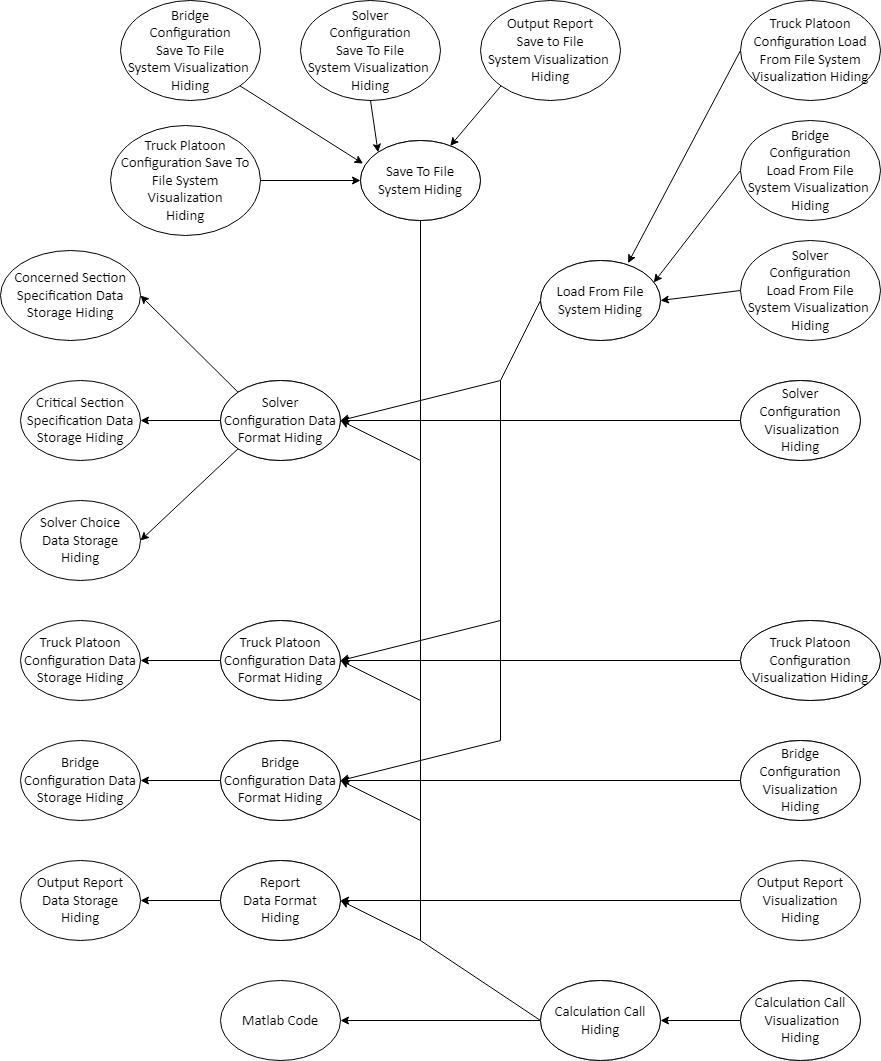
\includegraphics[width=1\textwidth]{../images/UseHierarchy.png}
\caption{Use hierarchy among modules}
\label{FigUH}
\end{figure}

%\section*{References}

\bibliographystyle {plainnat}
\bibliography{../../../refs/References}

\newpage{}

\end{document}